\documentclass[a4paper,12pt]{book}
\usepackage{graphicx}

\title{ISELL User Guide}
\author{Olcay Taner YILDIZ}

% vectors in bold math
\def\bc{{\mbox{\boldmath $c$}}}
\def\br{{\mbox{\boldmath $r$}}}
\def\bv{{\mbox{\boldmath $v$}}}
\def\bw{{\mbox{\boldmath $w$}}}
\def\bx{{\mbox{\boldmath $x$}}}
\def\bT{{\mbox{\boldmath $T$}}}

% matrices in bold 
\def\mS{{\bf S}}
\def\mA{{\bf A}}
\def\mW{{\bf W}}

% greek bold
\def\bSigma{{\mbox{\boldmath $\Sigma$}}}

% calligraphic
\def\cC{{\cal C}}
\def\cG{{\cal G}}
\def\cI{{\cal I}}
\def\cL{{\cal L}}
\def\cO{{\cal O}}
\def\cR{{\cal R}}
\def\cX{{\cal X}}

\def\sig{{\mbox{Sigmoid}}}

\def\bm{{\mbox{\boldmath $m$}}}
\def\bw{{\mbox{\boldmath $w$}}}
\def\bx{{\mbox{\boldmath $x$}}}
\def\mS{{\bf S}}
\def\bSigma{{\mbox{\boldmath $\Sigma$}}}

\begin{document}
\maketitle
\tableofcontents

\chapter{How to Compile \& Execute}
One needs only gcc to compile the ISELL program. Go to the source directory, and just write,
\begin{verbatim}
user@pc:~$make
\end{verbatim}
which will compile the ISELL C source code and creates isell executable program. The compilation is done with -ansi -pedantic options, therefore any programming struct or any nonstandard (ANSI standard) function call will result in an error in the compilation.

When you have the executable program, just write
\begin{verbatim}
user@pc:~$./isell
\end{verbatim}
to run the program. You can give an optional batch script file to the program. For example,
\begin{verbatim}
user@pc:~$./isell script.txt
\end{verbatim}
will run ISELL program, compiles and interprets the commands in the script.txt.

\chapter{External Files}
ISELL needs four files to operate. These are dictionary.txt, order.txt, hyperparameters.xml and parameters.xml.

\section{dictionary.txt}
This file contains functions written in the enhanced postscript (eps) language. The functions are
\begin{itemize}
\item[circle] Draws a circle to an eps file. It takes three parameters /y0, /x0 and /r representing the y and x axis coordinates of the center of the circle, and the radius of the circle respectively.
\item[cshow] Prints a string object as centred. It takes only the string as an argument.
\item[clshow] Prints a string object as left aligned. It takes only the string as an argument.
\item[crshow] Prints a string object as right aligned. It takes only the string as an argument.
\item[fillrect] Draws and fills a rectangle. It takes five parameters /upperY, /upperX, /lowerY, /lowerX and /gray representing the y and x axis coordinates of the upper-left corner of the rectangle, y and x axis coordinates of the lower-right corner of the rectangle and gray-scale depth of the color to fill with respectively.
\item[drawrect] Draws a rectangle. It takes four parameters /upperY, /upperX, /lowerY and /lowerX  representing the y and x axis coordinates of the upper-left corner of the rectangle, y and x axis coordinates of the lower-right corner of the rectangle respectively.
\item[xaxis] Draws the x axis. It takes five parameters /sameY, /secondX, /firstX, /tickwidth, and /tickcount representing y axis position of the x axis, start and end of the x axis, width of each tick and number of ticks to plot on the x axis respectively.
\item[yaxis] Draws the y axis. It takes five parameters /sameX, /secondY, /firstY, /tickwidth, and /tickcount representing x axis position of the y axis, start and end of the y axis, width of each tick and number of ticks to plot on the y axis respectively.
\item[verticalfill] Fills a rectangle by drawing vertical lines in it. It takes five parameters /upperY, /upperX, /lowerY, /lowerX, and /tickwidth representing the y and x axis coordinates of the upper-left corner of the rectangle, y and x axis coordinates of the lower-right corner of the rectangle and the distance
between two vertical lines respectively.
\item[horizontalfill] Fills a rectangle by drawing horizontal lines in it. It takes five parameters /upperY, /upperX, /lowerY, /lowerX, and /tickwidth representing the y and x axis coordinates of the upper-left corner of the rectangle, y and x axis coordinates of the lower-right corner of the rectangle and the distance between two horizontal lines respectively.
\item[squarefill] Fills a rectangle by drawing small squares in it. It takes five parameters /upperY, /upperX, /lowerY, /lowerX, and /tickwidth representing the y and x axis coordinates of the upper-left corner of the rectangle, y and x axis coordinates of the lower-right corner of the rectangle and the side length
of each small square respectively.
\item[dashedline] Draws a dashed line. It takes five parameters /secondY, /secondX, /firstY, /firstX, and /dashtype representing the y and x axis coordinates of the starting and ending points of the line and type of the dash respectively.
\item[line] Draws a usual line. It takes four parameters /secondY, /secondX, /firstY, /firstX, and /dashtype representing the y and x axis coordinates of the starting and ending points of the line respectively.
\end{itemize}

\section{command.txt}
This file contains the commands (and its properties) available in the ISELL program. The position of each command is important. In the process.c file, there is a function {\bf process\_order(int res)} which process each command in the interpreter (or batch script file). The parameter {\em res} corresponds to the index of the command and is the position of the command in the command.txt file. For example the command {\em exit} is the first command in the command.txt file and if {\em res} is 0, this command is processed.

There are 10 lines for each command in the command.txt file.
\begin{enumerate}
\item index. COMMAND
\item Name of the command. 
\item Group of the command. When the user enters the command help, the commands are grouped according to this field (and the subgroup) of the command. The program automatically groups the commands. Therefore if a nonexistent group is entered to this area, there will be no problem, it will be displayed correctly.
\item Subgroup of the command. The program automatically groups the commands. Therefore if a nonexistent subgroup is entered to this area, it will be displayed correctly.
\item Explanations of the return values of the command. Most commands in the ISELL environment return one (output variable of type real or integer such as out1, output variable of type string such as sout1) or more values (array output variable such as aout1, aout2, etc.) into the output variable(s). These output variables can be used as usual variables in the script.
\item Name of the output variables returned by this command.
\item Grammar of the command. This field of the command is used in compiling the script files. If the parameters of the command are not in the types as specified here, ISELL will return error 1016 in the compilation. Possible parameter types are $<$stringval$>$, $<$integerval$>$, and $<$realval$>$ for one string, integer, and real constant value (such as 3.4, 2) respectively; $<$stringvaln$>$, $<$integervaln$>$, and $<$realvaln$>$ for one or more string, integer, and real constant values respectively; $<$stringvar$>$, $<$integervar$>$, $<$realvar$>$, $<$filevar$>$, $<$matrixvar$>$ for string, integer, real, file, and matrix variables (such as i, j, st, myfile) respectively; $<$onoff$>$ for on or off constant value.
\item Explanations of the parameters of the command.
\item Explanation of the command itself (what it does, how it does, citation to the algorithm, etc.).
\item File name(s) of one or more example scripts. These example scripts can be found in the {\bf examples} directory.
\end{enumerate}

\subsection{To add a new command?}
\label{sec-addcommand}
In order to add a new command to the ISELL program follow the following steps:
\begin{enumerate}
\item Select a command name. Be sure there isn't another command with the same name.
\item Add 10 new lines to the end of the command.txt. Fill the lines with appropriate definitions, grammar and explanations. Remember ISELL will not open if the number of lines in the command.txt is not divisible by 10.
\item Add a new case to the switch in the {\bf process\_order} function. Be sure the number in the case is one less than the index of the new command.
\item If the command takes parameters (most of the time it does), call the {\bf checkparams} function. {\bf checkparams} will check if the user has given enough parameters to the command. First argument of the {\bf checkparams} function is always {\em paramcount} variable, which shows the number of parameters user has entered. Second argument of the {\bf checkparams} function is the number of parameters the command expects. Let say this number is $p$. Then there are $p$ more arguments of the {\bf checkparams} function which correspond to the error messages the user will see when he/she did't enter enough parameters. If the user did't enter first parameter, he/she will see the first message (Third argument of the checkparams function). If the user entered first parameter but did't enter the second parameter, he/she will see the second message (Fourth parameter of the checkparams function). In the ISELL program the error messages has their own codes. They are constant strings defined in messages.h file.
\item You can also check the type and bounds of the constant integer and real value parameters. Use {\bf atoi\_check} and {\bf atof\_check} functions for integer and real value parameters respectively. The third and fourth arguments of those functions are the minimum and maximum value allowed for the constant integer or real parameter.
\item Do not forget to set the output variable(s) if the command has it (them). Two main functions exist for this course namely {\bf set\_default\_variable} and {\bf set\_default\_string\_variable}.
\end{enumerate}

\section{hyperparameters.xml}
Most of the algorithms in the machine learning have hyperparameters to tune such as $k$ (nearest neighbor count) for nearest neighbor algorithm, $C$ for support vector machine algorithms, learning rate for gradient descent training as in neural networks or logistic regression. In ISELL, these hyperparameters can be tuned automatically using cross-validation. Before dividing into train or test sets, ISELL separates out some part of the original dataset (validation set) for hyperparameter tuning. {\em cvratio} is the command to set the percentage of the validation set. For each possible value of the hyperparameter, the training is done and the best hyperparameter value (the one that performs best on the validation set) is used for testing ({\bf tune\_hyperparameters\_of\_the\_supervised\_algorithm}). In order to tune hyperparameter of an algorithm, the script must contain line
\begin{verbatim}
hyperparametertune on
\end{verbatim}

For each hyperparameter there is a {\bf $<$parameter$>$} tag, which contains (i) name of the hyperparameter (ii) all possible values the hyperparameter can take as a sublist. Each possible value of the hyperparameter is surrounded by $<$value$>$, $<$/value$>$ tags. As an example:
\begin{verbatim}
<parameter name="k">
<value>1</value>
<value>2</value>
<value>3</value>
<value>4</value>
<value>5</value>
<value>6</value>
<value>7</value>
<value>8</value>
<value>9</value>
<value>10</value>
</parameter>
\end{verbatim}

\subsection{To add a new hyperparameter?}
In order to add a new hyperparameter to the ISELL program follow the following steps:
\begin{enumerate}
\item Select a name for the hyperparameter.
\item Add a new $<$parameter$>$ tag to hyperparameters.xml.
\item Add possible values of the new hyperparameter to hyperparameters.xml.
\item Modify {\bf tune\_hyperparameters\_of\_the\_supervised\_algorithm} function so that the specific algorithm can be run with hyperparameters tuned.
\item If the original algorithm does not need other validation data to use, one must add 
\begin{verbatim}
case ...:if (get_parameter_o("hyperparametertune") == ON)
           return YES;
         else 
           return NO;
\end{verbatim}
lines to {\bf is\_cvdata\_needed} function.
\end{enumerate}

\section{parameters.xml}

There are three classes of parameters in ISELL program. These are:
\begin{itemize}
\item The parameters of the learning algorithm such as $k$ (nearest neighbor count) for nearest neighbor algorithm, $C$ for support vector machine algorithms, learning rate for gradient descent training as in neural networks or logistic regression.
\item Parameters independent from the learning algorithm such as training and test set percentages (60 percent of the data will be for training, other for testing), number of folds (10 fold, 30 fold etc.), type of validation ($k$-fold crossvalidation, 5$\times$ 2 crossvalidation, 10$\times$ 10 crossvalidation, etc.), statistical test used in comparing classifiers or regressors (Wilcoxon sign-rank test, Sign test, Paired $t$ test, etc.).
\item Parameters of the ISELL program (most of them on-off type parameters) such as will the source code be displayed while it is running, will the results of the algorithms or tests etc. be displayed on the screen or forwarded to an output file.
\end{itemize}

The parameters can be in one of six types namely, INTEGER, FLOAT, STRING, ONOFF, LIST, and ARRAY.
\begin{itemize}
\item[INTEGER] The parameter can take integer values. Example parameters are: $nearcount$ (nearest neighbor count) for the nearest neighbor algorithm, $foldcount$ number of folds in crossvalidation, $precision$ floating-point precision in displaying real numbers on the screen or in a file, $maxhidden$ maximum number of hidden nodes in a hidden layer of multilayer percentron algorithm, $tailed$ type of statistical test two tailed (2) or one tailed (1), $perceptronrun$ number of epochs to train a gradient descent algorithm, $optimizecount$ number of optimization steps in RIPPER rule learning algorithm.
\begin{verbatim}
<parameter name="perceptronrun" type="INTEGER" value="10"/>
<parameter name="foldcount" type="INTEGER" value="2"/>
\end{verbatim}
\item[FLOAT] The parameter can take floating point values. Example parameters are: $learning\_rate$ initial learning rate used in training gradient descent algorithms, $confidencelevel$ confidence level of a statistical test to reject the null hypothesis, $noiselevel$ noise percentage used while producing noisy data, $svmC$, $svmnu$ C and nu parameters of the C-SVM (support vector machines) and nu-SVM learning algorithms, $testpercentage$ percentage of examples to put aside before dividing the data into training and validation sets, $cvratio$ percentage of the validation set with respect to the original dataset.
\begin{verbatim}
<parameter name="learning_rate" type="FLOAT" value="0.10"/>
<parameter name="variance_explained" type="FLOAT" value="0.99"/>
\end{verbatim}
\item[STRING] The parameter can take string values. Example parameters are: $imagefile$ when current figure will be saved this file name will be used, $modelfilename$ when the model of the current learning algorithm will be saved this file name will be used, $posteriorfilename$ when the posterior probabilities of the test instances will be saved this file name will be used.
\begin{verbatim}
<parameter name="testcodefilename" type="STRING" value=""/>
<parameter name="posteriorfilename" type="STRING" value=""/>
\end{verbatim}
\item[ONOFF] The parameter can take only on or off values. On and off values are stored as 1 and 0 in ISELL. Example parameters are: $timeon$ if it is on, the execution time of each command is reported, $displaycodeon$ if it is on, the program prints each line it is executing, $parallel$ if it is on, parallel programming (executing) is enabled, $accuracy$ if it is on, accuracy of the classification algorithms is reported, otherwise error is reported, $savetestfiles$ if it is on, the source code of the testing phase of the learning algorithm is saved in a given rogramming language (which is also a LIST type parameter), $hold$ same as hold on in the Matlab drawing environment, $showticks$ if it is on, ticks are displayed on the axes.
\begin{verbatim}
<parameter name="timeon" type="ONOFF" value="OFF"/>
<parameter name="displaycodeon" type="ONOFF" value="ON"/>
\end{verbatim}
\item[LIST] The parameter takes a value from a list of strings. Each string in the list is stored between $<$value$>$ and $<$/value$>$ tags. Example parameters are: $currentos$ operating system where ISELL program runs (it can take three different values as Windows, Solaris, Linux), $testtype$ name of the statistical test used is comparisons, $correctiontype$ name of the confidence level correction method, $modelselectionmethod$ name of the model selection technique, $prunetype$ name of the pruning algorithm used in decision tree pruning, $kerneltype$ type of kernel used in Support Vector Machines, $language$ name of the programming language.
\begin{verbatim}
<parameter name="correctiontype" type="LIST" value="bonferroni">
   <value>bonferroni</value>
   <value>holm</value>
   <value>nocorrection</value>
</parameter>
<parameter name="kerneltype" type="LIST" value="linear">
   <value>linear</value>
   <value>polynom</value>
   <value>rbf</value>
   <value>sigmoid</value>
</parameter>
\end{verbatim}
\item[ARRAY] The parameter is an array of values. Array elements can be INTEGER or FLOAT. $<$size$>$ tag represents the size of the array, $<$value$>$ tag represents default value of the elements of the array. Example parameters are: $hiddennodes$ number of hidden nodes in each hidden layer of the multilayer perceptron, $statecounts$ number of states in the Hidden Markov Model for each class.
\begin{verbatim}
<parameter name="hiddennodes" type="ARRAY" subtype="INTEGER" size="3" value="1"/>
<parameter name="svmcweights" type="ARRAY" subtype="FLOAT" size="50" value="1.0"/>
\end{verbatim}
\end{itemize}

\subsection{To add a new parameter?}
In order to add a new parameter to the ISELL program follow the following steps:
\begin{enumerate}
\item Select a name for the parameter. Be sure there isn't another parameter with the same name.
\item Add one or more lines to the parameters.xml file. If the parameter is of LIST type, add also all possible values. If the parameter is of ARRAY type, add the subtype and size of the array.
\item Specify the default value of the parameter in the $<$value$>$ tag.
\end{enumerate}
If the parameter is a changable parameter from the script, one needs add a new command (Section \ref{sec-addcommand}) in order to be able to change its value.

\chapter{Dataset Definition}
\label{sec-dataset}
In order to define a dataset or datasets to ISELL program, one needs first put all dataset directories in a single directory (data directory). Each dataset directory must contain at least one dataset file. The command to define the data directory is {\bf setdatadir}. For example, the partial script
\begin{verbatim}
setdatadir /home/olcay/datasets
\end{verbatim}
defines the data directory as /home/olcay/datasets. After defining the data directory, one loads a dataset definition file. The command for this purpose is {\bf loaddatasets}. For example, the partial script
\begin{verbatim}
loaddatasets mydataset.xml
\end{verbatim}
loads the datasets given in the file mydataset.xml. Here mydataset.xml must be a dataset definition file with a predefined format. An example mydataset.xml is given below:
\begin{verbatim}
<datasets>
<dataset name="iris" task="classification" size="150" 
         directory="iris" filetype="text" 
         separator="," filename="iris.data">
   <classes>
      <class value="iris-setosa" size="50"/>
      <class value="iris-versicolor" size="50"/>
      <class value="iris-virginica" size="50"/>
   </classes>
   <attributes>
      <attribute type="Real" available="True" min="4.3" max="7.9"/>
      <attribute type="Real" available="True" min="2.0" max="4.4"/>
      <attribute type="Real" available="True" min="1.0" max="6.9"/>
      <attribute type="Real" available="True" min="0.1" max="2.5"/>
      <attribute type="Output" available="True">
         <value>iris-setosa</value>
         <value>iris-versicolor</value>
         <value>iris-virginica</value>
      </attribute>
   </attributes>
</dataset>
</datasets>
\end{verbatim}
Although the tags and properties are self-explanatory we give the explanations below:
\begin{itemize}
\item[name] Name of the dataset
\item[task] Learning task for the dataset. Can be classification or regression.
\item[size] Number of instances in the dataset.
\item[directory] Name of the dataset directory that contains the dataset file.
\item[filetype] Only text files are supported for now.
\item[separator] The attributes in the dataset file are separated with a character. If the separator character is space just write " ".
\item[filename] Name of the dataset file.
\item[classes] The surrounding tag that contains the name of the classes and the number of instances in each class.
\item[attributes] The surrounding tag that contains the attributes.
\item[type] Type of the attribute. Three types of attributes are supported in ISELL. real
 integer and string (discrete) attributes. Output attribute has type output.
\item[min] Minimum value of the attribute.
\item[max] Maximum value of the attribute.
\item[available] Some attributes may be unusable in the learning.
\end{itemize}

\chapter{ISELL Script Language}

\section{Introduction}
We begin by considering a simple script.
\begin{verbatim}
'A first program in ISELL
writescreen Hello_World!
\end{verbatim}
Output:
\begin{verbatim}
Hello World!
\end{verbatim}

The line
\begin{verbatim}
'A first program in ISELL
\end{verbatim}
begins with \' indicates that this line is a {\em comment}. Comments in ISELL can not be extended by more than one line. 

The line
\begin{verbatim}
writescreen Hello_World!
\end{verbatim}
instructs the interpreter to print a string of characters. In ISELL language every statement must end
with the new line character. When the preceding writescreen command is executed, it prints the message Hello World! on the screen. The characters normally print exactly as they appear. Notice that the character '\_' was not printed on the screen. Since the parameters of every command are separated via space characters, in order to print space character one needs another character namely '\_'.

\subsection{Data Types and Variables}
Variables and constants are the basic data objects manipulated in a program. Declarations list the variables to be used, and state what type they have and perhaps what their initial values are. Operators specify what is to be done to them. Expressions combine variables and constants to produce new values. The type of an object determines the set of values it can have and what operations can be performed on it.

\subsubsection{Variable Names}
Variables are the basic data object in ISELL. They can be declared anywhere in the program and can only be used afterwards. The declaration of a variable is
\begin{center}
\framebox{data\_type variable\_name}
\end{center}
and the declaration of more than one variable is
\begin{center}
\framebox{data\_type variable\_name1 variable\_name2 $\ldots$ variable\_namen}
\end{center}

Sample variable definitions are given below:
\begin{verbatim}
integer x1 x2
real y
string st
file infile outfile
matrix m1 m2 mymatrix
\end{verbatim}

There are some restrictions on the names of variables.
\begin{enumerate}
\item Names are made up of letters and digits. So ab9c is a valid variable name, whereas ab[ not.
\item The underscore\index{underscore} can not be used inside a variable.
\item Upper case\index{uppercase} and lower case\index{lowercase} letters are not distinct, so x and X are the same.
\item Keywords are not reserved: You can use them as variable names.
\end{enumerate}

\subsubsection{Data types}
There are five basic data types in ISELL (given below).
\begin{table}[ht]
\begin{center}
\caption{Data types in ISELL}
\begin{tabular}{ll}
\hline
integer    & an integer \\
real  & double precision floating point \\
string & an array of characters \\
file & a file variable used in order to read and write text files\\
matrix & matrix variable \\
\hline
\end{tabular}
\end{center}
\end{table}

\subsubsection{Declarations}
All variables must be declared before use, although certain declarations can be made
explicitly by context. A declaration specifies a type, and contains a list of one or more
variables of that type, as in
\begin{verbatim}
integer lower upper step
string st
\end{verbatim}

Variables can be distributed among declarations in any fashion; the lists above could equally
well be written as
\begin{verbatim}
integer lower
integer upper
integer step
string st
\end{verbatim}

This latter takes more space, but is convenient for adding a comment to each declaration or for subsequent
modifications. A variable can not be initialized in its declaration. 

\subsection{Operators}
There are four types of operators in ISELL.
\begin{enumerate}
\item Arithmetic operators
\item Equality and relational operators
\item Assignment operators
\item Increment and decrement operators
\end{enumerate}

\subsubsection{Arithmetic Operators}
ISELL arithmetic operators are given below.  First four of them are regular arithmetic operators.
Addition, subtraction, multiplication and division. The fifth of them is the modulus operator,
which is the mod operation in mathematics. It gives the remainder when the first number is
divided by the second number.
\begin{table}[h!]
\begin{center}
\caption{ISELL arithmetic operators}
\begin{tabular}{lll}
\hline
Operation & Algebraic expression & ISELL expression \\
\hline
Addition & f+7 & f+7 \\
Subtraction &  p$-$c & p$-$c \\
Multiplication & bm & b*m \\
Division & $\frac{x}{y}$ & x/y \\
Modulus & r mod s & r@s \\
Power & $x^y$ & x\textasciicircum y \\
Logarithm & $\log_x y$ & x\textdollar y \\
\hline
\end{tabular}
\label{table_arithmetic_operators}
\end{center}
\end{table}

All operators can be applied to real and integer data types, whereas
there are only specific commands for file (Table \ref{table_file_commands}), matrix (Table \ref{table_matrix_commands}) and string (Table \ref{table_string_commands}) data types to operate on.

\begin{table}[h!]
\begin{center}
\caption{ISELL file commands}
\begin{tabular}{ll}
\hline
Command & Operation \\
\hline
openfile & Opens a file for reading or writing \\
closefile & Closes a file \\
writefile & Writes a string or a value to a file \\
readfile & Reads a value to a variable from a file \\
readarrayfile & Reads a group of values to a string array \\
\hline
\end{tabular}
\label{table_file_commands}
\end{center}
\end{table}

\begin{table}[h!]
\begin{center}
\caption{ISELL matrix commands}
\begin{tabular}{ll}
\hline
Command & Operation  \\
\hline
readposterior & Reads the posterior file into the matrix variable \\
readcposterior & Reads the posteriors of the correct class into \\
              & the matrix variable \\
mresize & Takes a list of columns and produces a new matrix which \\
        & contains only those columns \\
mcovariance & Takes the covariance of the first matrix and \\
            & returns it as the second matrix \\
mcorrelation & Takes the correlation of the first matrix and returns \\
             & it as the second matrix \\
meigenvectors & Finds the eigenvectors of the first matrix and returns it as \\
             & the rows of the second matrix in the order of \\
             & increasing eigenvalues \\
mtranspose  & Takes the transpose of the matrix \\
msum & Returns the sum of the elements of the matrix \\
mtrace & Returns the trace of a square matrix \\
mprint & Prints the given matrix to the given file \\
loadmatrix & Loads a matrix from a file \\
maverage & Finds the column averages of the matrix \\
mstdev & Finds the column standard deviations of the matrix \\
\hline
\end{tabular}
\label{table_matrix_commands}
\end{center}
\end{table}

\begin{table}[h!]
\begin{center}
\caption{ISELL string commands}
\begin{tabular}{ll}
\hline
Command & Operation \\
\hline
tokenize & Divides the input string into a list of tokens  \\
         & separated via a given list of characters \\
countchar & Returns number of occurences of a given character \\
          & in a given string variable \\
stringlength & Returns the length of a string variable \\
charatindex & Returns the character at the given position in the \\
            & given string variable \\
\hline
\end{tabular}
\label{table_string_commands}
\end{center}
\end{table}

\subsubsection{Equality and Relational Operators}

Although we make operations on variables and constants, we may also compare them. For this purpose, we use the equality and relational operators. These operators can be applied to integer, real and string data types. 
\begin{table}[h!]
\begin{center}
\caption{ISELL equality and relational operators}
\begin{tabular}{lll}
\hline
Operator & ISELL operator  & Meaning of ISELL condition \\
\hline
= & == or =  & x is equal to y \\
$\neq$ & != or $<>$ & x is not equal to y \\
$>$ & $>$ & x is greater than y \\
$<$ & $<$ &  x is less than y \\
$\geq$ & $>$=  & x is greater than or equal to y \\
$\leq$ & $<$=  & x is less than or equal to y \\
\hline
\end{tabular}
\label{table_relational_operators}
\end{center}
\end{table}

\subsubsection{Assignment Operators}

The operations such as
\begin{verbatim}
x = x + y
z = z - j
\end{verbatim}
where we add one variable to another variable or subtract one variable from another variable occurs so often in the programs that there are extra operators (assignment operators ) dedicated to them. With these
operators all of the arithmetic operators are extended to be assignment operators. So the examples above can be simplified as
\begin{verbatim}
x += y
z -= j
\end{verbatim}
Note that in ISELL assignments operators are commands, therefore they can only be used in prefix notation (Table \ref{table_assignment_operators}).

\begin{table}[h!]
\begin{center}
\caption{ISELL assignment commands}
\begin{tabular}{lll}
\hline
Assignment operator & Sample & Explanation \\
\hline
+= & += c 7 & c = c + 7 \\
$-$= & $-$= d 4 & d = d $-$ 4 \\
$*$= & *= e 5 & e = e * 5 \\
/= & /= f 3 & f = f / 3 \\
@= & @= g 9 & g = g mod 9 \\
\textasciicircum= & \textasciicircum= x 3 & $x = x^3$ \\
\textdollar= & \textdollar= y 4 & y = $\log_4 y$ \\
\hline
\end{tabular}
\label{table_assignment_operators}
\end{center}
\end{table}

\subsubsection{Increment and Decrement Operators}

In the looping, we usually add 1 to the loop variable (increment) or subtract 1 from the loop variable (decrement).
Since loops are one of the main structures of a program, in order to simplify the syntax of these sentences, ISELL has extra increment and decrement commands. For example  
\begin{verbatim}
++ c
-- b
\end{verbatim}
mean as
\begin{verbatim}
c = c + 1;
b = b - 1;
\end{verbatim}

\begin{table}[h!]
\begin{center}
\caption{ISELL increment and decrement operators}
\begin{tabular}{lll}
\hline
Operator & Sample & Explanation \\
\hline
++ & ++ a & Increment a by 1 \\
$--$ & $--$ b & Decrement b by 1 \\
\hline
\end{tabular}
\label{table_increment_decrement_operators}
\end{center}
\end{table}

\section{If-switch}

\subsection{If-else Structure}
\label{sec-if}

Let say we want to make a decision in the program, for example
we want to determine if a person's grade is greater than or equal to 60, and if it is so, to
print a message such as "Congrulations! You passed.".  We will do this in the program using an {\bf if}
statement as:
\begin{verbatim}
if >= grade 60
  writescreen Congrulations!_You_passed.
\end{verbatim}  
The syntax of the {\bf if-else} statement is:
\begin{center}
\fbox{
\begin{minipage}{10cm}
\begin{tabbing}
123\=\kill
if relational\_operator relational\_operand1 relational\_operand2 \\
\> $statementblock_1$ \\
else \\
\> $statementblock_2$ \\
endif
\end{tabbing}
\end{minipage}
}
\end{center}

{\bf Else} part of this statement is optional.

When the compiler runs this program first {\em expression} is evaluated; if it is true,
$statementblock_1$ is executed.  Otherwise if the expression is false, and there is an {\bf else} part, $statementblock_2$ is executed.
The code for each statementblock can be a null statement\index{null statement},
\begin{verbatim}
 if == x 4
 endif
\end{verbatim}  
or a single statement,
\begin{verbatim}
 if == y 4
   ++ y
 endif
\end{verbatim}
or a group of statements.
\begin{verbatim}
 if == x 4
   ++ y
   += z %y%
 endif
\end{verbatim}

The expression in the if statement is called a {\em condition}.  Each condition must be a single relational operation. A relational expression is formed by using the relational operators and the equality operators. (Discussed in the previous section). For example,
\begin{verbatim}
if > x 8
\end{verbatim}
is a conditional expression that checks if the variable \textsl{x} is larger than 8 or not. ISELL currently does not support complex relational expressions. 

\subsection{Switch}

Suppose you want to run C4.5 algorithm on 4 datasets ({\em iris}, {\em vote}, {\em mushroom}, and {\em bupa}). Your code will be as:
\begin{verbatim}
if = algindex 1
  c45 iris cv 1
else 
  if = algindex 2
    c45 vote cv 1
  else
    if = algindex 3
      c45 mushroom cv 1
    else
      c45 bupa cv 1
    endif
  endif
endif
\end{verbatim}

This multi-way decision can be more easily done with the reserved word {\bf switch}.
The {\bf switch} statement is a multi-way decision that tests whether an expression matches one of a number of constant integer values, and branches accordingly.  The syntax of {\bf switch} is:
\begin{center}
\fbox{
\begin{minipage}{10cm}
\begin{tabbing}
123\=456\=\kill
switch variable \\
\> case $constant\_expression_1$ \\ 
\> \> $statements_1$ \\
\> case $constant\_expression_2$ \\
\> \> $statements_2$ \\
\> $\ldots$ \\
endswitch \\
\end{tabbing}
\end{minipage}
}
\end{center}
If value of the variable is equal to $constant\_expression_1$, then all $statements_1$ will be executed and the program continues after the {\bf endswitch}. If expression is equal to $constant\_expression_2$, then all $statements_2$ will be executed and the program continues after the {\bf endswitch}. If expression is not equal to none of the constant expressions, none of the statements will be executed and again the program continues after the {\bf endswitch}.

Now our example program can be done with switch as follows:\\
\begin{verbatim}
switch algindex 
  case 1
    = dataset iris
  case 2 
    = dataset vote
  case 3
    = dataset mushroom 
  case 4
    = dataset bupa
endswitch
c45 %dataset% cv 1
\end{verbatim}
Some comments for switch:
\begin{itemize}
\item Each {\bf case} is labeled by one constant or constant expression. In the example program, 1, 2, 3, and 4 are integer-valued constants.
\item If a {\bf case} matches the expression value, execution starts at that case. For example, if \textsl{algindex} is 2, the execution starts at
\begin{verbatim}
= dataset vote
\end{verbatim}
\item All {\bf case} expressions must be different. 
\item Cases can occur in any order. So in the example program you can exchange the positions of cases 1, 2, 3, and 4. 
\end{itemize}

\section{Loops}

\subsection{Repetition Structures}
Most programs involve repetition or {\em looping}. A {\em loop} is a group of instructions the computer executes repeatedly while
some {\em loop-continuation condition} remains true. There are two types of repetition:
\begin{enumerate}
\item Counter-controlled repetition
\item Sentinel-controlled repetition
\end{enumerate}

Counter-controlled repetition is sometimes called {\em definite repetition} because we know in advance exactly how many times the loop will be executed. On the other hand, sentinel-controlled repetition is sometimes called {\em indefinite repetition} because it is not known in advance how many times the loop will be executed.

In counter-controlled repetition, a {\em control variable} is used to count the number of repetitions.  The control variable is incremented or decremented (usually by 1) each time the group of instructions is performed.  When the value of the control variable indicates that the correct number of repetitions has been performed, the loop terminates and the computer continues executing with the statement after the repetition structure.

Counter-controlled repetition requires:
\begin{enumerate}
\item The {\em name} of the control variable (or loop counter)
\item The {\em initial\index{initial} value} of the control variable
\item The {\em increment} (or {\em decrement}) by which the control variable is modified each time through the loop.
\item The condition that tests for the {\em final value} of the control variable (i.e., whether looping should continue).
\end{enumerate}

Sentinel values are used to control repetition when:
\begin{enumerate}
\item The precise number of repetitions is not known in advance, and
\item The loop includes statements that obtain data each time the loop is performed.
\end{enumerate}

The sentinel value indicates ``end of data". The sentinel is entered after all regular data items have been supplied to the program. Sentinels must be distinct from regular data items. For example, if the user will enter positive numbers, the sentinel can be any nonpositive value.

\subsection{While statement}
{\bf While} statement has the following syntax:
\begin{center}
\fbox{
\begin{minipage}{10cm}
\begin{tabbing}
123\=\kill
while relational\_operator relational\_operand1 relational\_operand2 \\
\> statementblock \\
endwhile
\end{tabbing}
\end{minipage}
}
\end{center}

In this {\bf while} structure, first the relationals expression is evaluated (See Section \ref{sec-if}).  If it is true, statementblock is executed and expression is re-evaluated. This cycle continues until expression becomes false, at which point execution resumes after statement. Let say we want to sum all numbers between 1 and 10 and print the result. The code will be
\begin{verbatim}
integer counter sum
= sum 0
= counter 1
while <= counter 10
  += sum %counter%
  ++ counter
endwhile 
writescreen %sum%
\end{verbatim}

Output:
\begin{verbatim}
55
\end{verbatim}

This sample program prints the sum of the numbers from 1 to \textsl{counter}, where \textsl{counter} goes from 1 to 10. The declarations
\noindent
\begin{verbatim}
  integer counter sum
  = counter 1
\end{verbatim}
{\em names} the control variable\index{control variable}, declares it to be integer and sets it to an {\em initial value} of 1.

The statement
\noindent
\begin{verbatim}
  ++ counter
\end{verbatim}
increments the loop counter by 1 each time the loop is performed.  The loop-continuation condition\index{loop-continuation condition} 
\begin{verbatim}
  <= counter 10
\end{verbatim} 
in the {\bf while} structure tests if the value of the control variable is less than or equal to 10 (the last value for which the condition is true).

\subsection{For statement}
{\bf For} statement has the following syntax:
\begin{center}
\fbox{
\begin{minipage}{10cm}
\begin{tabbing}
123\=\kill
for $loop\_control\_variable$ $expression_1$ $expression_2$ \\
\> statementblock \\
endfor $loop\_control\_variable$
\end{tabbing}
\end{minipage}
}
\end{center}

$expression_1$ initializes the loop's control variable, $expression_2$ is the loop-continuation condition. The {\bf for} repetition structure handles all the details of counter-controlled repetition\index{counter-controlled repetition}. We can write our example program now with for:
\noindent
\begin{verbatim}
integer counter sum
= sum 0
for counter 1 10
  += sum %counter%
endfor counter
writescreen %sum%
\end{verbatim}
\noindent

The program operates as follows. When the {\bf for} structure begins to execute, the control variable \textsl{counter} is initialized to 1.  Then, the loop-continuation condition \textsl{counter}$<$=10 is checked.  Because the initial value of \textsl{counter} is 1, the condition is satisfied so \textsl{sum} is incremented by \textsl{counter} and assignment operator add the value of \textsl{counter} to \textsl{sum}.  The control variable \textsl{counter} is then incremented by 1, and the loop begins again with the loop-continuation test.  This process continues until the fail of the loop-continuation test (when \textsl{counter} is 11) and repetition terminates.

Some comments for {\bf for} loop:
\begin{enumerate}
\item The initialization and loop-continuation condition can contain arithmetic expressions.
\item The increment may be negative (in which case you must add a fifth parameter -1 to the for statement)
\item If the loop-continuation condition is initially false, the body portion of the loop is not performed. Instead, execution proceeds with the statement following the for structure.
\end{enumerate}

\subsection{Nested loops}
The loops that we have seen so far can also be nested. With two loops nested, we can have two or more {\bf for} loops or {\bf while} loops. If two loops are nested, to finish one step of the outer loop, one must finish all the steps of the inner loop. Therefore, if the outer loop mas $m$ steps and the inner loop has $n$ steps, the statements in the inner loop will be executed $mn$ times, whereas the statements out of the inner loop but in the outer loop are executed $m$ times.

In the nested loop example, we want to run KNN algorithm (with $k$ = 3) 100 times (with different train and test sets) on 4 datasets ({\em iris}, {\em vote}, {\em mushroom}, and {\em bupa}).
\begin{verbatim}
integer i j
string dataset
nearcount 3
for i 1 4
  switch i
    case 1
      = dataset iris
    case 2
      = dataset vote
    case 3
      = dataset mushroom
    case 4
      = dataset bupa
  endswitch
  for j 1 100
    knn %dataset% cv %j%
  endfor j
endfor i
\end{verbatim}
The outer loop counts each number between 1 and 4 and sets the dataset name accordingly. The inner loop runs knn algorithm 100 times for the datasets selected in the outer loop.

\section{Arrays}

\subsection{Arrays}
An array is a  group of memory locations. These locations are related by the fact
that they have all the same name and the same type. To refer to a particular location
or element within the array, we specify the name of the array and the position number
of the particular element within the array.

Let see an example array \textsl{c} (Table \ref{ex-array}). This array contains twelve
elements. Any one of these elements may be referred to by giving the name of the array
followed by the position number of the particular element in square brackets([]).
Thus, the first element of array \textsl{c} is referred to as \textsl{c}[1], the second element of array \textsl{c} is referred to as \textsl{c}[2], in general the \textsl{i}'th element of array \textsl{c} is referred to as \textsl{c}[\textsl{i}].

\begin{table}[ht]
\begin{center}
\caption{An example array c}
\label{ex-array}
\begin{tabular}{ll}
\hline
c[1] & -2 \\
c[2] & 23 \\
c[3] & -100 \\
c[4] & 1 \\
c[5] & 0 \\
c[6] & 3 \\
c[7] & -245 \\
c[8] & 6 \\
c[9] & 34 \\
c[10] & 12 \\
c[11] & 7 \\
c[12] & 34 \\
\hline
\end{tabular}
\end{center}
\end{table}

The position number is usually called subscript\index{subscript}. The subscript may be an integer or an
integer expression. For example, if \textsl{a} = 5 and \textsl{b} = 6, then the statement
\begin{verbatim}
+= c[%a+b%] 2
\end{verbatim}
results in array element \textsl{c}[11] being incremented by 2.

Also to divide the value of the seventh element of array \textsl{c} by 2 and assign the result to variable \textsl{x},
we would write
\begin{verbatim}
= x %c[6]/2%
\end{verbatim}

\subsection{Declaring Arrays}
Arrays occupy space in memory. We specify the number of allocations required by each array, so that the
computer reserves memory for each array. The syntax for array declaration is
\begin{center}
\framebox{elementtype\_type array\_name[array\_size]}
\end{center}
For example, to tell the computer reserve 12 elements for integer array \textsl{c}, the
declaration
\begin{verbatim}
integer c[12]
\end{verbatim}
is used. Array variables can also be declared with a single declaration 
\begin{center}
\framebox{elementtype\_type array\_name1[array\_size1] array\_name2[array\_size2] $\ldots$}
\end{center}
such as
\begin{verbatim}
integer b[100] x[27]
\end{verbatim}
It is important to remember that arrays are automatically initialized to zero by ISELL. 

Let see an example, which compute the sum of the elements of the array.
\begin{verbatim}
integer a[100] i sum
for i 1 100
  = a[i] %i%
endfor i
= sum 0
for i 1 100
  += sum %a[i]%
endfor i
writescreen %sum%
\end{verbatim}
\noindent
Output:
\begin{verbatim}
5050
\end{verbatim}
In this example program, array \textsl{a} is declared with 100 elements and initialized as \{1, 2, 3, $\ldots$, 100\}. In order to take the sum of the elements of array \textsl{a}, one must add all elements of array \textsl{a} (\textsl{a}[1], \textsl{a}[2], \ldots, \textsl{a}[100]) to \textsl{sum}. We can do this by making a loop and by setting the loop counter to count from 1 to 100.

\subsection{Multidimensional Arrays}
Arrays in ISELL can have multiple dimensions. For example, we use two dimensional array to represent
tables of values consisting of information in rows and columns. To identify a particular
element of such a table, we must specify two subscripts. The first identifies the row
in which the element is contained, and the second identifies the column in which the element
is contained. Let see an example of a two dimensional array \textsl{c}.

\begin{table}[ht]
\label{ex-twoarray}
\caption{An example two dimensional array \textsl{c}}
\begin{tabular}{lllll}
\hline
 & Column 1 & Column 2 & Column 3 & Column 4 \\
\hline
Row 1 & c[1,1] & c[1,2] & c[1,3] & c[1,4] \\
Row 2 & c[2,1] & c[2,2] & c[2,3] & c[2,4] \\
Row 3 & c[3,1] & c[3,2] & c[3,3] & c[3,4] \\
\hline
\end{tabular}
\end{table}

Every element in the array \textsl{c} is identified by an element name of the form \textsl{c}[\textsl{i},\textsl{j}] \textsl{c} is the name of the array, and \textsl{i} and \textsl{j} are the subscripts that uniquely identify each element in \textsl{c}.

All elements of a multidimensional array is initialized to zero automatically like a onedimensional array. 

We now give three examples, where the first example is adding two matrices, the second example is multiplying these two matrices and the third example is transposing a matrix.

\noindent
Addition:
\begin{verbatim}
integer i j
integer a[10,10] b[10,10] c[10,10]
for i 1 10
  for j 1 10
    = c[i,j] %a[i,j]+b[i,j]%
  endfor j
endfor i
\end{verbatim}
To add two matrices, we add the elements of those two matrices one by one. Therefore, the \textsl{i},\textsl{j}'th element of the resulting \textsl{c} array is equal to the sum of the \textsl{i},\textsl{j}'th elements of the arrays \textsl{a} and \textsl{b}.

\noindent
Multiplication:
\begin{verbatim}
integer i j k total
integer a[10,10] b[10,10] c[10,10]
for i 1 10
  for j 1 10
    = total 0
    for k 1 10
      += total %a[i,k]*b[k,j]%
    endfor k
    = c[i,j] %total%
  endfor j
endfor i
\end{verbatim}
The \textsl{i},\textsl{j}'th element of the resulting array \textsl{c} is obtained by summing up the products of the row \textsl{i} of the array \textsl{a} and the column \textsl{j} of the array \textsl{b}.

\noindent
Transpose:
\begin{verbatim}
integer i j
for i 1 10
  for j 1 10
    = b[i,j] %a[j,i]%
  endfor j
endfor i
\end{verbatim}
The \textsl{i},\textsl{j}'th element of the resulting array \textsl{b} is equal to the \textsl{j},\textsl{i}'th element of the array \textsl{a}.

\chapter{Operating System Commands}

Some of the operating systems commands can be used in ISELL. These commands are given in Table \ref{shell-commands}.

\begin{table}[ht]
\label{shell-commands}
\caption{Operating system commands available in ISELL}
\begin{tabular}{ll}
\hline
Command & Explanation \\
\hline
cls or reset & Clear the screen\\
copy or cp & Copies one file to a given file \\
cd & Change current directory to the given directory \\
del or rm & Delete(s) one or more files \\ 
dir or ls & Lists contents of the current directory \\
move or mv & Moves (renames) one file to another file \\
rename & Changes the name of the given file to another \\
mkdir & Creates a new directory \\
rmdir & Removes the given directory \\
\hline
\end{tabular}
\end{table}

\chapter{Distributions \& Statistical Tests}

\section{Probability Distributions}
Probability distributions can be categorized into two as discrete and continuous probability distributions. Each probability distribution is founded on a probability density function, which is the probability that the variable X coming from that probability distribution has the value of x. For discrete distributions, this value can be calculated as single point probability but for continuous distributions it has to be expressed in terms of an integral between two points.

\subsection{Normal Distribution}

The probability density function for normal distribution is,
\begin{equation}
f(x)=\frac{1}{\sqrt{2\pi}\sigma}e^{-\frac{(x-\mu)^2}{2\sigma^2}}
\end{equation}
If $\mu=0$ and $\sigma=1$, it is called {\em standard normal distribution}. To convert normal distribution to standard normal distribution, we subtract the mean and divide to the square root of the variance. The parameters, mean and variance are,
\begin{eqnarray}
E[X]=\mu \nonumber \\
Var[X]=\sigma^2
\end{eqnarray}

Many statistical tests are based on the assumption that the data comes from a normal distribution. Central limit theorem states that the sum of independent and identically distributed random variables approaches to normal distribution as the sample size becomes large (usually larger than 30). The sum of normally distributed random variables is also normally distributed.

There is also a connection between random numbers generated using uniform distribution and normal distribution. By summing 12 randomly generated numbers and subtracting 6, we get a standard normally distributed random variable.

Sample Script:
\begin{verbatim}
>>normal 2.0
0.977
>>normal 1.0
0.841
>>normalinv 0.95
1.645
>>normalinv 0.99
2.326
\end{verbatim}

\subsection{Chi Square Distribution}
The probability density function for chi square distribution is,
\begin{equation}
f(x)=\frac{e^\frac{-x}{2}x^{{\frac{v}{2}}-1}}{2^\frac{v}{2}\Gamma(\frac{v}{2})}
\end{equation}
where $v$ is the degree of freedom of the chi square distribution and $\Gamma$ is the Gamma function. The parameters, mean and variance are,
\begin{eqnarray}
E[X]=v \nonumber \\
Var[X]=\sqrt{2v}
\end{eqnarray}

The sum of squares of $N$ normally distributed random variables is chi-square distributed with N degrees of freedom. 

\begin{equation}
\chi_n = {\cal N}_1 + {\cal N}_2 + \ldots + {\cal N}_n
\end{equation}

The sum of $N$ chi-square distributed random variables is also chi-square distributed. The sum of the degrees of freedoms of the $N$ random variables will be the degree of freedom of the resulting random variable.

\begin{equation}
\chi_{v_1 + v_2 + \ldots + v_n} = \chi_{v_1} + \chi_{v_2} + \ldots + \chi_{v_n}
\end{equation}

Sample Script:
\begin{verbatim}
>>chi 2.0 3
0.572
>>chi 2.0 5
0.849
>>chiinv 0.05 2
5.991
>>chiinv 0.01 2
9.210
\end{verbatim}

\subsection{F Distribution}
Probability density function for F distribution is,
\begin{equation}
f(x)=\frac{\Gamma(\frac{v_1+v_2}{2})(\frac{v_1}{v_2})^{\frac{v_1}{2}}x^{{\frac{v_1}{2}}-1}}{\Gamma(\frac{v_1}{2})\Gamma(\frac{v_2}{2})(1+\frac{v_1x}{v_2})^{\frac{v_1+v_2}{2}}}
\end{equation}
where $v_1$ and $v_2$ are degrees of freedom of the F distribution and $\Gamma$ is the Gamma function. The parameters, mean and variance are,
\begin{eqnarray}
E[X]=\frac{v_2}{v_2-2} \nonumber \\
Var[X]=\sqrt{\frac{2v_2^2(v_1+v_2-2)}{v_1(v_2-2)^2(v_2-4)}}
\end{eqnarray}

F distribution is the ratio of two chi-square distributions with degrees of freedom $v_1$ and $v_2$ respectively, where each chi-square is first divided by its degree of freedom.

\begin{equation}
F_{v_1, v_2} = \frac{\frac{\chi_{v_1}}{v_1}}{\frac{\chi_{v_2}}{v_2}}
\end{equation}

If $v_2=1$, then F distribution value is equal to the square of the t distribution's value with $v_1$ degrees of freedom.

\begin{equation}
F_{v_1, 1} = t_{v_1}^2
\end{equation}

Sample Script:
\begin{verbatim}
>>f 2.0 5 10
0.164
>>f 3.0 5 10
0.066
>>finv 0.05 5 10
3.326
>>finv 0.01 5 10
5.636
\end{verbatim}

\subsection{t Distribution}
The probability density function for t distribution is,
\begin{equation}
f(x)=\frac{(1+\frac{x^2}{v})^{-\frac{v+1}{2}}}{B(0.5,0.5v)\sqrt{v}}
\end{equation}
where $v$ is the degree of freedom of the t distribution and $B$ is the Beta function. The parameters, mean and variance are,
\begin{eqnarray}
E[X]=0 \nonumber \\
Var[X]=\sqrt{\frac{v}{v-2}}
\end{eqnarray}

t distribution approaches to normal distribution as $v$ gets larger.

Sample Script:
\begin{verbatim}
>>t 1.0 10
0.170
>>t 2.0 10
0.037
>>tinv 0.05 10
1.812
>>tinv 0.01 10
2.764
\end{verbatim}

\section{Statistical Tests}

Statistical tests in the literature can be divided into two groups. Parametric tests and nonparametric tests.

In parametric methods, there is usually an assumption on the underlying distribution of the data. Most parametric methods are based on normality assumption because the theory behind the test can only be verified with the normal distribution. One problem with parametric methods is that we can not be sure about the underlying probability distribution, which is usually normal distribution. One way to overcome this problem is to perform hypothesis tests on classifiers' error rates to detect nonnormality.

In contrast to parametric methods, nonparametric methods do not assume a particular population probability distribution, which makes them valid for any population with any probability distribution. When the data is discrete, we can only use nonparametric methods.

Second type of grouping of statistical tests divides tests into three parts. Pairwise tests, range tests and multiple tests. These types of tests differ from each other on the number of classifiers they compare. Pairwise comparison methods compare two classifiers at a time, multiple comparison methods can compare all classifiers at once and range tests can compare any number of classifiers between two and $K$.

For each of the tests we say that, we have $K$ classifiers on which we make $N$-fold crossvalidation, where each classifier is tested on $N$ validation sets. So we have $K\times N$ results and let $Y_{ij}$ represents the number of errors model $i$ does on validation set $j$. Each classifier has a mean of $m_i, i=1, 2, \ldots, k$. All of the classifiers have a general mean of $m$. For parametric tests we assume that, all of the $K$ samples are independent and normally distributed. There is no such an assumption for nonparametric tests.

When we compare classifiers by using statistical tests, we will use the data given below. This data contains four classifiers and there are 10 trials for each classifier. 

\begin{table}[h!]
\label{example}
\begin{center}
\caption{Example error percentages of four classifiers}
\begin{tabular}{cccc}
\hline
error1.txt & error2.txt & error3.txt & error4.txt \\
\hline
9  & 15 & 18 & 21 \\
11 & 13 & 16 & 19 \\
10 & 17 & 15 & 17 \\
13 & 14 & 17 & 23 \\
8  & 15 & 13 & 18 \\
12 & 16 & 15 & 20 \\
10 & 15 & 14 & 16 \\
11 & 17 & 17 & 21 \\
7  & 14 & 15 & 21 \\
10 & 13 & 16 & 19 \\
\hline
\end{tabular}
\end{center}
\end{table}

\subsection{One-Way Anova Test}

\subsubsection{Hypothesis}
The null hypothesis of this test is  
\begin{center}
$H_0: m_1=m_2=\ldots=m_K$
\end{center}
against the alternative
\begin{center}
$H_1$: At least one of the samples has a larger or smaller mean than at least one of the other
samples
\end{center}

\subsubsection{Method}
The method starts by calculating MST as
\begin{equation}
MST=N\frac{\sum_{i=1}^K(m_i-m)^2}{K-1}
\end{equation}
This is the total standard error between the means of the classifiers. We calculate MSE as
\begin{equation}
MSE=\frac{\sum_{i=1}^K\sum_{j=1}^N(Y_{ij}-m_i)^2}{KN-K}
\end{equation}
which is total mean square error. If $\frac{MST}{MSE}$ ratio is smaller than the F distribution value with $K-1$ and $KN-K$ degrees of freedom, then $H_0$ is accepted. Otherwise it is rejected.

\subsubsection{Assumptions}
\begin{itemize}
\item All samples are independent and composed of normal random variables with unknown mean $\mu_i$
and unknown variance $\sigma^2$.
\end{itemize}

Sample Script:
\begin{verbatim}
anova error1.txt error2.txt error3.txt error4.txt
\end{verbatim}

\subsection{K-Fold Paired t Test}
The name of this test comes from the fact that first it uses k-fold cross-validation, second it pairs test errors of the classifiers and third it uses t distribution.

\subsubsection{Hypothesis}
The null hypothesis of this test is  
\begin{center}
$H_0: m_1=m_2$
\end{center}
against the alternative
\begin{center}
$H_1$: One of the classifiers has larger or smaller error than the other.
\end{center}

\subsubsection{Method}
$p_i$ is the difference between the error rates of the two classifiers as
$p_i=Y_{1i}-Y_{2i}$. 

The estimator for mean
\begin{equation}
m=\frac{\sum_{i=1}^kp_i}{k}
\end{equation}
and variance
\begin{equation}
S^2=\frac{\sum_{i=1}^k(p_i-m)^2}{k-1}
\end{equation}

We calculate the test statistic
\begin{equation}
L=\frac{\sqrt{k}m}{S}
\end{equation}

The null hypothesis is accepted with $\alpha$ level of confidence, if this value is between $-t_{\alpha /2,k-1}$ and $t_{\alpha /2,k-1}$, otherwise it is rejected.

\subsubsection{Assumptions}
\begin{itemize}
\item The difference of the classifier's errors on the test set is approximately normally distributed
with zero mean and unknown variance $\sigma^2$.
\end{itemize}

\subsubsection{Sample Script}
\begin{verbatim}
cvttest error1.txt error2.txt
\end{verbatim}

\subsection{5$\times$2 cv t Test}
This test is proposed by \cite{dietterich98}. In this test five replications of 2--fold cross--validation are performed. 

\subsubsection{Hypothesis}
The null hypothesis of this test is
\begin{center}
$H_0: m_1=m_2$
\end{center}
against the alternative
\begin{center}
$H_1$: One of the classifiers has larger or smaller test error than the other.
\end{center}

\subsubsection{Method}
$p_i^{(j)}$ is the difference between the error rates of the two classifiers as
$p_i^{1}=Y_{1(2i-1)}-Y_{2(2i-1)}$ and $p_i^{2}=Y_{1(2i)}-Y_{2(2i)}$. $s_i^2$ is the estimated
variance of the $i$'th replication as $s_i^2=(p_i^{(1)}-\bar{p_i})^2+(p_i^{(2)}-\bar{p_i})^2$.

Total variance is then 
\begin{equation}
VAR=\sum_{j=1}^5s_i^2
\end{equation}
Now the null hypothesis $H_0$ is accepted with $\alpha$ level of confidence if the value $\frac{p_i^{1}}{\sqrt{\frac{VAR}{5}}}$ is between $-t_{\alpha / 2, 5}$ and $t_{\alpha / 2, 5}$. Otherwise it is rejected.

\subsubsection{Assumptions}
\begin{itemize}
\item The difference of the classifier's errors on the test sets, is treated as approximately normally distributed
with zero mean and unknown variance $\sigma^2$.
\item $p_i^{(1)}$ and $p_i^{(2)}$ are independent normals.
\item Each of the estimated variances $s_i^2$ are assumed to be independent.
\item $p_i^{(1)}$ and the sum of the variances of the differences are independent of each other. 
\end{itemize}

\subsubsection{Sample Script}
\begin{verbatim}
tpaired5x2 error1.txt error2.txt
\end{verbatim}

\subsection{5$\times$2 cv F Test}
This test first appeared in \cite{alpaydin99}. It is a variant of the previous version 
5$\times$2 cv t test. This version of the test has lower Type I
error and higher power.

\subsubsection{Hypothesis}
The null hypothesis of this test is  
\begin{center}
$H_0: m_1=m_2$
\end{center}
against the alternative
\begin{center}
$H_1$: One of the classifiers has larger or smaller test error than the other.
\end{center}

\subsubsection{Method}
We have $n=10$ in this test. 10 comes from 5x2 cross validation, five replications of 2--fold cross--validation.
$p_i^{(j)}$ is the difference between the error rates of the two classifiers as
$p_i^{1}=Y_{1(2i-1)}-Y_{2(2i-1)}$ and $p_i^{2}=Y_{1(2i)}-Y_{2(2i)}$. $s_i^2$ is the estimated
variance for each of the five replication as $s_i^2=(p_i^{(1)}-\bar{p_i})^2+(p_i^{(2)}-\bar{p_i})^2$.

To test this, first we calculate sum of squares of $p_i^{(j)}$'s:
\begin{equation}
DIFFS=\sum_{i=1}^5\sum_{j=1}^2(p_i^{(j)})^2
\end{equation}
Second we calculate sum of variances of five replications
\begin{equation}
VAR=2\sum_{j=1}^5s_i^2
\end{equation}
Now the null hypothesis $H_0$ is accepted with $\alpha$ level of confidence, if $\frac{DIFFS}{VAR}$ is smaller than the probability value of F distribution with degrees of freedoms 10, 5 and $\alpha$ level of confidence.

\subsubsection{Assumptions}
\begin{itemize}
\item The difference of the classifier's errors on the test sets, is treated as approximately normally distributed
with zero mean and unknown variance $\sigma^2$.
\item $p_i^{(1)}$ and $p_i^{(2)}$ are independent normals.
\item Each of the estimated variances $s_i^2$ are assumed to be independent.
\item The sum of squares of the differences of the error rates and sum of the variances of the differences are independent of each other. 
\end{itemize}

\subsubsection{Sample Script}
\begin{verbatim}
ftest error1.txt error2.txt
\end{verbatim}

\subsection{Newman-Keuls Test}
The design and probability distribution used is the same as Tukey's procedure.
But the form of the test is changed. This test is first proposed by Newman(1939). Later in 1952, Keuls proposed the same test in another journal, Euphytica.

\subsubsection{Hypothesis}
The null hypothesis of this test is that all means in a subset of $L$ means are equal  
\begin{center}
$H_0: m_1=m_2=\ldots=m_L$
\end{center}
against the alternative
\begin{center}
$H_1$: At least one of the samples has a larger or smaller mean than at least one of the other
samples in a subset $L$ samples of $K$ samples of data.
\end{center}

If $H_0$ is rejected, we make comparisons on all the means and find which means are significantly different from each other.

\subsubsection{Method}
The basic idea in multiple range tests is comparing the best and the worst of the subset of classifiers selected. If they are not significantly different from each other, then we can say that all of the classifiers between this two methods are also not significantly different.

To be able to do that, we first put the classifiers means in increasing order. We then test for equality of $K$ means, after $K-1$ means, $K-2$ means until $2$ means. But at each time when we compare $L$ means, we only make $K-L+1$ tests. First we check the equality of means $m_1$ and $m_L$, then $m_2$ and $m_{L+1}$, $\ldots$, $m_{K-L+1}$ and $m_K$.

If $L$ means are equal to each other, then we do not need to make any further comparisons between these means. 
So we do not have to control any of the subsets of the means between $m_i$ and $m_j$, when $m_i$ and $m_j$ are not significantly different from each other.

The comparisons of $m_i$ and $m_j$ is done by subtracting the two means and comparing the difference with
$q_{K(N-1),M}^{0.95}\sqrt{\frac{MSE}{N}}$, where $M$ is the number of means in the subset compared, $q_{f_1,f_2}^{\alpha}$ is the studentized 
range distribution with $\alpha$ confidence and $f_1$, $f_2$ degrees of freedom. If the difference
is smaller than the calculated number we accept the null hypothesis, otherwise we reject it.

\subsubsection{Assumptions}
\begin{itemize}
\item $Y_{1i}$ and $Y_{2i}$ are normally distributed random variables with means $\mu_i$ and a common variance $\sigma^2$.
\end{itemize}

\subsubsection{Sample Script}
\begin{verbatim}
newmankeuls error1.txt error2.txt error3.txt error4.txt
\end{verbatim}

\subsection{Sign Test}
The sign test is one of the nonparametric oldest tests. It was first used in 18th century to compare the number of males born with the number of females born in 82 years in England. The aim of the sign test is to check for equality of the number of positive examples with the number of negative examples. If one can separate the data into two groups of examples, sign test could be applied.

\subsubsection{Hypothesis}
The hypothesis of this test is that the number of positive examples are equal to the number of negative examples.

\begin{center}
$H_0: P(+)=P(-)$
\end{center}
against the alternative
\begin{center}
$H_1$: $P(+)\neq P(-)$.
\end{center}

\subsubsection{Method}
The data consists of observations of a bivariate random sample $(X_1, Y_1)$, $(X_2, Y_2)$, $\ldots$, $(X_n, Y_n)$, where there are $N$ examples. Within each pair $(X_i, Y_i)$ a comparison is done and each pair is classified as '+' if $X_i > Y_i$, '--' if $X_i < Y_i$ and 0 if $X_i = Y_i$. Number of positive examples are represented as P(+), number of negative examples are represented as $P(-)$ and total number of examples are represented as $P(+) + P(-) = N$. The test statistic uses snadard normal distribution with $\alpha / 2$ level of confidence. Test statistic t is given as:
\begin{equation}
t = \frac{1}{2}(n + z_{\alpha/2}\sqrt{n})
\end{equation}
If $P(+)$ is between $t$ and $N - t$, then the null hypothesis is accepted, otherwise the null hypothesis is rejected.

\subsubsection{Assumptions}
\begin{itemize}
\item The bivariate random variables $(X_i, Y_i)$ are mutually independent.
\item Each pair $(X_i, Y_i)$ may be represented as positive, negative or 0.
\end{itemize}

\subsubsection{Sample Script}
\begin{verbatim}
signtest error1.txt error2.txt
\end{verbatim}

\subsection{Wilcoxon Rank Test}
This test first appeared in Wilcoxon (1945) for equal sample sizes and generalized in Mann and Whitney (1947) for unequal sample sizes.

\subsubsection{Hypothesis}
The hypothesis of this test is   
\begin{center}
$H_0: m_1=m_2$
\end{center}
against the alternative
\begin{center}
$H_1$: One of the classifiers has larger or smaller test error than the other.
\end{center}

\subsubsection{Method}
To make this test, first the ranks of the results of the classifiers $R_{ij}$ (the rank of the $j$'th trial of
the $i$'th classifier) must be determined. To give ranks, we order all of the $Y_{ij}$'s, and give the best one the first rank, the second best one the second rank etc. If ties occur, we give the average rank to all $Y_{ij}$s. After finding ranks, we find the sum of the ranks of the first classifier, $T_1$.
\begin{equation}
T_1=\sum_{i=1}^NR_{1i}
\end{equation}
If there are ties in the data, we get new $T_L$ by using the following formula:
\begin{equation}
T_1=\frac{T_1-N\frac{2N+1}{2}}{\sqrt{\frac{N^2}{2N(2N-1)}\sum_{i, j}R_{ij}-\frac{N^2(2N+1)^2}{4(2N-1)}}}
\end{equation}
By using $T_1$ we get the following statistic:
\begin{equation}
S=\frac{T_1+0.5-\frac{N(2N+1)}{2}}{\sqrt{\frac{N^2(2N+1)}{12}}}
\end{equation}
If S is between $-z_{\alpha / 2}$ and $z_{\alpha / 2}$, then the null hypothesis is accepted with $\alpha$ level of confidence, otherwise it is rejected.

\subsubsection{Assumptions}
\begin{itemize}
\item Both samples are random samples from their respective populations.
\item There is independence within each sample and between the two samples.
\end{itemize}

\subsubsection{Sample Script}
\begin{verbatim}
wilcoxon error1.txt error2.txt
\end{verbatim}

\subsection{Kruskal-Wallis Test}
The Wilcoxon test for two samples was extended to include more than two samples by Kruskal and Wallis (1952).
This test can be used with unequal samples sizes.

\subsubsection{Hypothesis}
The hypothesis of this test is
\begin{center}
$H_0: m_1=m_2=\ldots=m_K$
\end{center}
against the alternative
\begin{center}
$H_1$: At least one of the samples has a larger or smaller mean than at least one of the other
samples
\end{center}

\subsubsection{Method}
The ranks $R_{ij}$ are assigned to the examples as in Wilcoxon test. The test statistic is calculated as:
\begin{equation}
T=\frac{12}{KN(KN+1)}\sum_{i=1}^K\frac{R_i^2}{N}-3(KN+1)
\end{equation}
,where $R_i$ is the sum of ranks of the $i$'th classifier and $\sum_{i=1}^KR_i=\frac{KN(KN+1)}{2}$.

If there are ties in the dataset, test statistic is defined as:
\begin{equation}
T=\frac{1}{S^2}(\sum_{i=1}^k\frac{R_i^2}{n_i}-\frac{N(N+1)^2}{4})
\end{equation}
where $S^2$ is,
\begin{equation}
S^2=\frac{1}{N-1}(\sum_{i, j}R(X_{ij})^2-N\frac{(N+1)^2}{4})
\end{equation}

We test the null hypothesis by comparing this value with chi-square distribution with $K$-1 degrees of freedom.
If the value is smaller than the chi-square distribution value, we accept the null hypothesis, otherwise we reject it.

\subsubsection{Assumptions}
\begin{itemize}
\item All samples are random samples from their respective populations.
\item There is independence within each sample and among the various samples.
\end{itemize}

\subsubsection{Sample Script}
\begin{verbatim}
kruskalwallis error1.txt error2.txt error3.txt error4.txt
\end{verbatim}

\subsection{Van Der Waerden Test}
Van Der Waerden (1952/1953) proposed another comparison of $K$ samples as in Kruskal-Wallis test.
This test can also be used with unequal sample sizes.

\subsubsection{Hypothesis}
The hypothesis of this test is  
\begin{center}
$H_0: m_1=m_2=\ldots=m_K$
\end{center}
against the alternative
\begin{center}
$H_1$: At least one of the samples has a larger or smaller mean than at least one of the other
samples
\end{center}

\subsubsection{Method}
Like Kruskal-Wallis test, we calculate ranks $R_{ij}$ of the examples. We convert each rank $R_{ij}$
into the $\frac{R_{ij}}{KN+1}$ quantile of a standard normal random variable.
\begin{equation}
A_{ij}=the \frac{R_{ij}}{KN+1}'th\ quantile
\end{equation}
We calculate the mean of these $A_{ij}$ for each classifier as:
\begin{equation}
\hat{A_i}=\frac{1}{N}\sum_{j=1}^NA_{ij}
\end{equation}
The variance of these scores is
\begin{equation}
S^2=\frac{1}{KN-1}\sum_{KN}A_{ij}^2
\end{equation}
The test statistic is defined as
\begin{equation}
T=\frac{1}{S^2}\sum_{i=1}^KN\hat{A_i}^2
\end{equation}

We test the null hypothesis by comparing this value with chi-square distribution with $K$-1 degrees of freedom.
If the value is smaller than the chi-square distribution value, we accept the null hypothesis, otherwise we reject it.

\subsubsection{Assumptions}
\begin{itemize}
\item All samples are random samples from their respective populations.
\item There is independence within each sample and among the various samples.
\end{itemize}

\subsubsection{Sample Script}
\begin{verbatim}
vanderwaerdan error1.txt error2.txt error3.txt error4.txt
\end{verbatim}

\chapter{Supervised Learning}

\section{Experimental Setup}
To run a supervised learning algorithm, first you need to set the datasets directory ({\bf setdatadir} command) then load the datasets ({\bf loaddatasets} command). To see how these commands work, see Chapter \ref{sec-dataset}.

In ISELL, you can run a supervised algorithm in three ways:
\begin{enumerate}
\item[Cross-validation] In $k$ fold cross-validation, the dataset is divided into $k$ equal parts. To generate a train set and validation set pair, we keep one of the $k$ parts out as the validation set and combine the remaining $k - 1$ parts to produce the training set. If we do this for each of the $k$ different parts, we get $k$ training and validation set pairs. An example script for $k$ fold cross-validation is:
\begin{verbatim}
runcount 1
foldcount 10
c45 iris cv 1
\end{verbatim}
If you want 5$\times$2 cross-validation \cite{dietterich98}, you will use {\bf runcount} command to make 5 times 2-fold cross-validation. For example:
\begin{verbatim}
runcount 5
foldcount 2
nearcount 3
knn vote cv 1
\end{verbatim}
will run K-nearest neighbor algorithm with $K$ = 3 on {\em vote} dataset  using 5$\times$2-fold cross-validation.
\item[Bootstrap] Another cross-validation technique is {\em bootstrap} \cite{efron79}. The basic idea is to randomly draw datasets with replacement from the training set where each sample contains the same number of instances as the training set. This is done $K$ times producing $K$ bootstrap datasets. An example script for $k$ bootstrap is:
\begin{verbatim}
runcount 100
nearestmean bupa bootstrap 1
\end{verbatim}
will run 100 times nearest-mean algorithm on {\em bupa} dataset using bootstrap sampling technique.
\item[Single train and test set] If you have your training and test set pairs ready, you can also use ISELL to train the supervised algorithm on your training set and test on your test set. To do this, just write:
\begin{verbatim}
logistic mushroom mytrain.txt mytest.txt
\end{verbatim}
will train logistic regression on mytrain.txt train set and will test on mytest.txt test set, where both files are formatted according to the {\em mushroom} dataset.
\end{enumerate}

You can also separate some part of the dataset as a test set before doing any bootstrap or cross-validation. ISELL will then test the algorithm not on the validation set (for cross-validation) but on the test set. In this case, there is only one test set, but since there are 10 different training sets, there will be 10 different classifiers (regressors) and each will be tested on this single test set to produce 10 error rate. Use {\bf testpercentage} command for this purpose. For example:
\begin{verbatim}
testpercentage 0.333333
runcount 1
foldcount 10
c45 iris cv 1
\end{verbatim}
will separate 1/3 part of the dataset as the test set, then will do 10-fold crossvalidation on the remaining 2/3 part of the dataset.

To save the outputs (error rate, confusion matrix, etc.) of the supervised algorithm, you can use the following commands:
\begin{itemize}
\item[output] When you run a supervised algorithm on a dataset, the expected error(s) are written on the screen. In order to forward these errors to an output file, you can use the output command. For example:
\begin{verbatim}
output error.txt
runcount 1
foldcount 10
c45 iris cv 1
\end{verbatim} 
will run C4.5 algorithm on {\em iris} dataset and will print the errors on 10 folds to the output file error.txt. Opening a new output file will close the previous output file automatically.
\item[printposterior]
\item[posteriorfile] If you are running a classification algorithm, you may not only want the expected error but also the posterior probabilities for each class of each test instance. In order to print the posterior probabilities use {\bf printposterior} (set to {\bf on}) and set the {\bf posteriorfile} to the posterior output file. For example:
\begin{verbatim}
output error.txt
printposterior on
posteriorfile posterior.txt
runcount 1
foldcount 10
c45 iris cv 1
\end{verbatim} 
\item[printconfusion]
\item[confusionfile] If you are running a classification algorithm, you may not only want the expected error but also the confusion matrix. In order to print the confusion matrix use {\bf printconfusion} (set to {\bf on}) and set the {\bf confusionfile} to the confusion output file. For example:
\begin{verbatim}
output error.txt
printconfusion on
confusionfile confusion.txt
runcount 1
foldcount 10
c45 iris cv 1
\end{verbatim} 
\item[savemodel]
\item[modelfile] You can also save the model (if you are running $k$-fold crossvalidation $k$ models) of the supervised learning algorithm. Use {\bf savemodel} (set to {\bf on}) and set the {\bf modelfile} to the model output file. For example:
\begin{verbatim}
output error.txt
savemodel on
modelfile model.txt
runcount 1
foldcount 10
c45 iris cv 1
\end{verbatim}
Then you can run {\bf testmodel} command to test the saved model on a separate test set. For example:
\begin{verbatim}
testmodel modelfile newtest.txt
\end{verbatim}
will test the model saved before (10 decision trees) on newtest.txt test set.
\end{itemize}

\section{Classification Algorithms}

\subsection{SELECTMAX}
SELECTMAX decides based on the prior class probability without looking at the input. No parameters.

\subsection{NEARESTMEAN}
NEARESTMEAN keeps the mean vector of the features for each class and chooses the class with the nearest mean using Euclidean distance \cite{alpaydin04}. No parameters.

\subsection{GAUSSIAN}
GAUSSIAN is the parametric classifier where each class is represented by a Gaussian and a common covariance matrix is shared by all classes \cite{alpaydin04}. No parameters.

\subsection{NAIVEBAYES}
NAIVEBAYES is the classic classifier where each feature is assumed to be Gaussian distributed \cite{alpaydin04} and each feature is independent from other features. No parameters.

\subsection{QDACLASS}
QDACLASS is parametric classifier where each class is represented by a Gaussian and covariance matrices are different for each class \cite{alpaydin04}. No parameters.

\subsection{C4.5RULES}
C4.5RULES starts with the C4.5 tree and converts it to a rule set by writing each path from the root to a leaf as a rule. The initial rule set therefore has as many rules as there are leaves in the tree \cite{quinlan93}. These generated rules may contain superfluous conditions and may cause overfitting. C4.5Rules prunes rules by removing those conditions whose removal do not increase the error rate on the training set. After pruning the conditions in the rules, the best subset of the rules is searched according to MDL \cite{quinlan89}. The search is exhaustive if the number of rules is small (less than or equal to ten), otherwise it is done by best first search starting from ten different subsets of rules. No parameters.

\subsection{KNN}
KNN is the nearest-neighbor classification algorithm \cite{duda73}. Number of nearest neighbors are set using {\bf nearcount} command.

\subsection{C45}
C45 is the archetypal decision tree method \cite{quinlan93}. A decision tree is made up of internal decision nodes and terminal leaves. The input vector is composed of $d$ attributes, $\bx=[x_1, \ldots, x_d]^T$, and the aim in classification is to assign $\bx$ to one of $K$ mutually exclusive and exhaustive classes, $\cC_1, \ldots, \cC_K$. Each internal node $m$ implements a decision function, $f_m(\bx)$, where each branch of the node corresponds to one outcome of the decision. Each leaf of the tree carries a class label. In {\em univariate} decision trees (for example in C4.5), the decision at internal node $m$ uses only one attribute, i.e., one dimension of $\bx$, $x_j$. 

Type of pruning is set using {\bf prunetype} command. If type of pruning is pre-pruning, we need a data size threshold, because, in pre-pruning, the tree is not fully constructed until zero training error but is kept simple by early termination. At any node, if the dataset reaching that node is small, even if it is not pure, it is not further split and a leaf node is created instead of growing a subtree. This threshold is set using {\bf pruningthreshold} command.

\subsection{LDT}
LDT is Linear discriminant tree algorithm. The details of the algorithm are given in \cite{yildiz04}. The parameters are the same as C4.5.

\subsection{LDACLASS}
LDACLASS is the Multiple Discriminant Analysis classifier \cite{duda73}. If the covariance matrix is singular, Principal Component Analysis (PCA) is used to decrease dimensionality. The percentage of variance explained in PCA is set using {\bf variance\_explained} command.

\subsection{LOGISTIC}
LOGISTIC is the linear logistic discriminator trained to minimize cross-entropy by gradient-descent. Discrete features are converted to numeric features by 1-of-$n$ encoding. Initial learning rate is set using {\bf learningrate} command. Number of epochs is set using {\bf perceptronrun} command. After each epoch, the learning rate is decreased by multiplying it with a constant factor. This factor is set using {\bf etadecrease} command.

\subsection{IREP, IREP2, RIPPER}
IREP, IREP2 and RIPPER are rule learning algorithms. RIPPER learns rules from scratch starting from an empty rule set. It has two phases: In the first phase, it builds an initial set of rules, one at a time, and in the second phase, it optimizes the rule set $m$ times, typically twice \cite{cohen95}. 

In the first phase, RIPPER learns rules one by one. First, propositional conditions are added one at a time to a rule, at each step choosing the condition that maximizes the information gain. Choosing the best is done exhaustively by  searching all possible split points ($x_i<\theta$ or $x_i\geq\theta$ for numeric features and $x_i = v$ for discrete features). When we insert a new condition, the coverage of the rule (number of instances that a rule covers) decreases, since some of the examples that are covered by the rule do not obey the new condition. We stop adding conditions further, when the current rule does not cover any negative examples. 

The rule is then pruned to alleviate overfitting. Conditions are removed one by one, where each time the condition that mostly increases a rule value metric (based on the accuracy on the prune set) is selected for removal. We stop removing conditions when the rule value metric can not be increased further. 

RIPPER uses MDL and in RIPPER, rules are added to a rule set to minimize the total description length. The total description length of a rule set is the number of bits to represent the rules plus the number of bits needed to identify the exceptions to the rules in the training set. We stop adding rules when the total description length of the rule set is larger than 64 bits from the minimum description length obtained so far or if the error rate of the new rule is larger than 0.5. 

In the second phase, rules in the rule set are optimized. Two alternatives are grown for each rule. The first candidate, the replacement rule, is grown starting with an empty rule,  whereas the second candidate, the revision rule, is grown starting with the current rule. These two rules and the original rule are compared and the one with the smallest description length is selected and put in place of the original rule. 

RIPPER learns rules to separate a positive class from a negative class. A $(K>2)$-class problem is converted into a sequence of $K-1$ two-class problems. This is done first by sorting classes in the order of increasing prior probabilities. In order to solve the $i$th two-class problem, $i=1,\ldots,K-1$, $C_i$ is taken as the positive class and the union of classes $C_{i+1}$, $C_{i+2}$, $\ldots$, $C_K$ is taken as the negative class. For each two-class problem, there are the two phases of learning a rule set and optimizing it, as we discussed above. We therefore generate a sequence of rules and the most probable class is the final default rule without conditions and it matches any instance which is not covered by any previous rule.

Number of optimization steps are set using {\bf optimizecount} command.

\subsection{RBF}
RBF is the Radial Basis Function network classification algorithm \cite{alpaydin04}. Number of Gaussians are set using {\bf hiddennodes} command. Initial learning rate is set using {\bf learningrate} command. Number of epochs is set using {\bf perceptronrun} command. After each epoch, the learning rate is decreased by multiplying it with a constant factor. This factor is set using {\bf etadecrease} command. If momentum is used, set alpha parameter of the momentum using {\bf alpha} command.

\subsection{MLPGENERIC}
MLPGENERIC is the well-known multilayer perceptron classification algorithm, where one can train the neural network with any number of hidden layers (from zero that is linear perceptron). Number of hidden nodes in each layer is set using {\bf hiddennodes} command. Initial learning rate is set using {\bf learningrate} command. Number of epochs is set using {\bf perceptronrun} command. After each epoch, the learning rate is decreased by multiplying it with a constant factor. This factor is set using {\bf etadecrease} command. If momentum is used, set alpha parameter of the momentum using {\bf alpha} command.

\subsection{DNC}
DNC \cite{ash89dynamic} builds MLP networks for classification with a single hidden layer. It starts with small number of hidden units and incrementally adds hidden nodes to the network until a satisfactory solution is found. Hidden nodes are added one at a time and to the same hidden layer. The weights of the newly added hidden node are initialized randomly to a small number. The whole network (both the old hidden nodes and the new one) is re-trained after each addition. The decision of adding a new hidden node is made by considering the flatness of the average error curve. Number of hidden nodes in each layer is set using {\bf hiddennodes} command. Initial learning rate is set using {\bf learningrate} command. Number of epochs is set using {\bf perceptronrun} command. After each epoch, the learning rate is decreased by multiplying it with a constant factor. This factor is set using {\bf etadecrease} command. If momentum is used, set alpha parameter of the momentum using {\bf alpha} command. Error threshold, error drop ratio and the window size parameters of the DNC algorithm are set with {\bf errorthreshold}, {\bf errordropratio} and {\bf windowsize} commands.

\subsection{MULTILDT}
MULTILDT is the multivariate tree where each decision node is linear \cite{yildiz00} and uses all inputs as opposed to a univariate decision tree, such as C4.5. When the inputs are correlated, looking at one feature may be too restrictive. A {\em linear multivariate tree}, at each internal node, uses a linear combination of all attributes. 
\begin{equation}
f_m(\bx): \bw_m^T \bx + w_{m0} = \sum_{j=1}^d w_{mj} x_j + w_{m0} > 0
\end{equation}
To be able to apply the weighted sum, all the attributes should be numeric and discrete values need be represented numerically (usually by 1-of-$L$ encoding) before. The weighted sum returns a number and the node is binary. In this linear case, each decision node divides the input space into two with a hyperplane of arbitrary orientation and position where successive decision nodes on a path from the root to a leaf further divide these into two and the leaf nodes define polyhedra in the input space. The parameters are the same as C4.5. For PCA when required, variance explained is set using {\bf variance\_explained} command.

\subsection{OMNILDT}
OMNILDT is the omnivariate decision tree algorithm \cite{yildiz01}. In omnivariate decision tree, at each node, we train and compare all three possible nodes; univariate, linear multivariate, and nonlinear multivariate, and using a statistical test, we choose the best and continue tree induction recursively. Each node implements a binary split to induce simple and interpretable trees. To group $K>2$ classes into two, we use Guo and Gelfand's \cite{guo92} exchange heuristic which uses class information.

\subsection{SVM, NUSVM}
SVM (or NUSVM) is the Support vector machine classifier with different type of kernels. The source code is exported from the LIBSVM 2.82 library \cite{libsvm}. C (or nu), Sigma, gamma and bias values are set using {\bf svmC} (or {\bf svmnu}), {\bf sigma}, {\bf svmgamma}, and {\bf svmcoef0} commands respectively. Kernel type is set using {\bf kerneltype} command and if the kernel is poynom kernel, the degree of the polynomial kernel is set using {\bf svmdegree} command.

\section{Regression Algorithms}

\subsection{ONEFEATURE}
ONEFEATURE finds the best axis-aligned split $x_i < c$. Using that split, the training instances are divided into two parts. For each part, the estimated output value is calculated by taking the average of the output values. This is a regression stump with only one node and two leaves. No parameters.

\subsection{SELECTAVERAGE}
SELECTAVERAGE finds the average of the output values of the training data. It uses this value as the estimated output value for all test cases. This the regression version of SELECTMAX. No parameters.

\subsection{LINEARREG}
LINEARREG is the classic linear regression algorithm. No parameters.

\subsection{QUANTIZEREG}
QUANTIZEREG divides each input feature into ten equal-sized bins to generate hyperrectangles in the instance space and calculates the average output in each bin. To combat the curse of dimensionality, Principal Component Analysis (PCA) is used to decrease dimensionality to two and regressogram is applied in this two dimensional space. Number of bins are set using {\em partitioncount} command.

\subsection{KNNREG}
KNNREG is the nearest-neighbor regression algorithm \cite{duda73}. Number of nearest neighbors are set using {\bf nearcount} command.

\subsection{GPROCESSREG}
GPROCESSREG does Gaussian process regression as described in \cite{bishop95}. Sigma, gamma and bias values are set using {\bf sigma}, {\bf svmgamma}, and {\bf svmcoef0} commands respectively. Kernel type is set using {\bf kerneltype} command and if the kernel is poynom kernel, the degree of the polynomial kernel is set using {\bf svmdegree} command.

\subsection{RBFREG}
RBF is the Radial Basis Function network regression algorithm \cite{alpaydin04}. Number of Gaussians are set using {\bf hiddennodes} command. Initial learning rate is set using {\bf learningrate} command. Number of epochs is set using {\bf perceptronrun} command. After each epoch, the learning rate is decreased by multiplying it with a constant factor. This factor is set using {\bf etadecrease} command. If momentum is used, set alpha parameter of the momentum using {\bf alpha} command.

\subsection{MLPGENERICREG}
MLPGENERIC is the well-known multilayer perceptron regression algorithm, where one can train the neural network with any number of hidden layers (from zero that is linear perceptron). Number of hidden nodes in each layer is set using {\bf hiddennodes} command. Initial learning rate is set using {\bf learningrate} command. Number of epochs is set using {\bf perceptronrun} command. After each epoch, the learning rate is decreased by multiplying it with a constant factor. This factor is set using {\bf etadecrease} command. If momentum is used, set alpha parameter of the momentum using {\bf alpha} command.

\subsection{DNCREG}
DNC \cite{ash89dynamic} builds MLP networks for regression with a single hidden layer. It starts with small number of hidden units and incrementally adds hidden nodes to the network until a satisfactory solution is found. Hidden nodes are added one at a time and to the same hidden layer. The weights of the newly added hidden node are initialized randomly to a small number. The whole network (both the old hidden nodes and the new one) is re-trained after each addition. The decision of adding a new hidden node is made by considering the flatness of the average error curve. Number of hidden nodes in each layer is set using {\bf hiddennodes} command. Initial learning rate is set using {\bf learningrate} command. Number of epochs is set using {\bf perceptronrun} command. After each epoch, the learning rate is decreased by multiplying it with a constant factor. This factor is set using {\bf etadecrease} command. If momentum is used, set alpha parameter of the momentum using {\bf alpha} command. Error threshold, error drop ratio and the window size parameters of the DNC algorithm are set with {\bf errorthreshold}, {\bf errordropratio} and {\bf windowsize} commands.

\subsection{SVMREG, NUSVMREG}
SVMREG (or NUSVMREG) is the Support vector machine regressor with different type of kernels. The source code is exported from the LIBSVM 2.82 library \cite{libsvm}. C (or nu), p, Sigma, gamma and bias values are set using {\bf svmC} (or {\bf svmnu}), {\bf svmp}, {\bf sigma}, {\bf svmgamma}, and {\bf svmcoef0} commands respectively. Kernel type is set using {\bf kerneltype} command and if the kernel is poynom kernel, the degree of the polynomial kernel is set using {\bf svmdegree} command.

\chapter{Graphics Environment}

\section{Plot Commands}

\begin{itemize}
\item[plotx] Plots one dimensional data.
\begin{verbatim}
plotx data1.txt
legendposition none
\end{verbatim}
\includegraphics[width=\linewidth]{graphics1.eps}

Another example:
\begin{verbatim}
plotx data1.txt
hold on
plotx data2.txt
legendposition none
\end{verbatim}
\includegraphics[width=\linewidth]{graphics2.eps}
\item[plotxy] Plots two dimensional data.
\begin{verbatim}
plotxy data3.txt
legendposition none
\end{verbatim}
\includegraphics[width=0.5\linewidth]{graphics3.eps}

Another example:
\begin{verbatim}
plotxy data3.txt
hold on
plotxy data4.txt
legendposition none
\end{verbatim}
\includegraphics[width=0.5\linewidth]{graphics4.eps}
\item[plotxyline] Plots two dimensional data and draws lines between neighbor points.
\begin{verbatim}
plotxyline data5.txt red 1
legendposition none
\end{verbatim}
\includegraphics[width=0.5\linewidth]{graphics5.eps}

Another example:
\begin{verbatim}
plotxyline data5.txt red 1
hold on
plotxyline data6.txt blue 2
legendposition none
\end{verbatim}
\includegraphics[width=0.5\linewidth]{graphics6.eps}
\item[plotxynames] Plots two dimensional data where each point is labeled with a given name
\begin{verbatim}
plotxynames data8.txt
\end{verbatim}
\includegraphics[width=0.5\linewidth]{graphics16.eps}

\item[polyplot] Plots a given polynomial between two values
\begin{verbatim}
polyplot -1 1 x2+x+1 red
legendposition none
\end{verbatim}
\includegraphics[width=0.5\linewidth]{graphics7.eps}

Another example:
\begin{verbatim}
polyplot -1 1 x+1 red
hold on
polyplot -1 1 x2+x+1 blue
polyplot -1 1 x3+x2+x+1 green
polyplot -1 1 x4+x3+x2+x+1 black
legendposition none
\end{verbatim}
\includegraphics[width=0.5\linewidth]{graphics8.eps}

\item[plotay] Plots dataset and error (or accuracy) information
\begin{verbatim}
plotay data7.txt
legendposition none
\end{verbatim}
\includegraphics[width=0.5\linewidth]{graphics9.eps}

\item[plotmv] Plots mean and standard deviation of the files
\begin{verbatim}
plotmv 1.c45 1.knn 1.lda 1.lp
xaxisnames iris
\end{verbatim}
\includegraphics[width=0.5\linewidth]{graphics10.eps}

Another example:
\begin{verbatim}
plotmv 1.c45 1.knn 1.lda 1.lp
hold on
plotmv 2.c45 2.knn 2.lda 2.lp
plotmv 3.c45 3.knn 3.lda 3.lp
xaxisnames iris dermatology breast
\end{verbatim}
\includegraphics[width=0.5\linewidth]{graphics11.eps}

\item[boxplot] Draws the boxplot of the files
\begin{verbatim}
boxplot 1.c45 1.knn 1.lda 1.lp
xaxisnames iris
\end{verbatim}
\includegraphics[width=0.5\linewidth]{graphics12.eps}

Another example:
\begin{verbatim}
boxplot 1.c45 1.knn 1.lda 1.lp
hold on
boxplot 2.c45 2.knn 2.lda 2.lp
boxplot 3.c45 3.knn 3.lda 3.lp
xaxisnames iris dermatology breast
\end{verbatim}
\includegraphics[width=0.5\linewidth]{graphics13.eps}

\item[boxplot] Draws the histogram plot of the files
\begin{verbatim}
histplot 1.c45 1.knn 1.lda 1.lp
xaxisnames C4.5 KNN LDA LP
yaxisnames iris
\end{verbatim}
\includegraphics[width=0.5\linewidth]{graphics14.eps}

Another example:
\begin{verbatim}
histplot 1.c45 1.knn 1.lda 1.lp
hold on
histplot 2.c45 2.knn 2.lda 2.lp
histplot 3.c45 3.knn 3.lda 3.lp
xaxisnames C4.5 KNN LDA LP
yaxisnames iris dermatology breast
\end{verbatim}
\includegraphics[width=0.5\linewidth]{graphics15.eps}

\item[plotgauss] Plots gaussian fits for the data in the file
\begin{verbatim}
plotgauss 1.c45
hold on
plotgauss 1.knn
plotgauss 1.lda
plotgauss 1.lp
legendnames C4.5 KNN LDA LP
\end{verbatim}
\includegraphics[width=\linewidth]{graphics17.eps}

\end{itemize}

\bibliography{references}
\bibliographystyle{IEEEtran}

\end{document}
